\documentclass[]{article}
\usepackage{graphicx}
\usepackage{fancyhdr}
\usepackage{listings}
\usepackage{url}
\usepackage[top=3cm,bottom=3cm,left=3.5cm,right=3.5cm,footskip=1.5cm,headheight=1.5cm,headsep=.5cm,textheight=3cm]{geometry}

\pagestyle{fancy}
\lhead{ACS Java component and Apache Commons SCXML integration}

\frenchspacing

\title{
	% The two figures on the top
   
\includegraphics[width=0.30\linewidth,height=!]{img/csrg}
   \hfill
   
\includegraphics[width=0.2\linewidth,height=!]{img/eso-logo}\\
	\vspace{2cm}
	%The current title
   \emph{ACS Java component and Apache Commons SCXML integration} \\
   \vspace{1cm}Technical Review
}
\date{}

\begin{document}

\maketitle
\thispagestyle{empty}

%\begin{center}
\hspace{-3.3cm}
\hfill
\begin{tabular}{|p{0.4\linewidth}|p{0.20\linewidth}|p{0.20\linewidth}|p{0.35\linewidth}|} \hline
\textbf{Authors} & \textbf{Organization} & \textbf{Date} &
\textbf{Notes}\\
\hline\hline
Cristian Morales & UTFSM & February 8 \\
\hline
\end{tabular}
\hfill
%\end{center}

\clearpage
\cfoot{}
\thispagestyle{fancy}
\cfoot{\thepage}
\setcounter{page}{1}
\tableofcontents
\clearpage

\section{Introduction}

This document describes the steps to create an ACS Java component integrated with the Apache SCXML Engine.

Commons SCXML \cite{Apache} provides a generic event-driven state machine based execution environment (based on CCXML and Harel State Tables) borrowing the semantics defined by SCXML and defining a language that can be used in many ways. Most things that can be represented as an UML state chart (business process flows, view navigation bits, interaction or dialog management, and too many more to list here ) can leverage the Commons SCXML library.

The example described is an extension of the one used in the first review document \cite{GoogleCode} with additional features implemented using API's advanced elements, which allow to extend or alter the semantics of the state machine document. The original model was a use case derived from the Apache Commons website \cite{Apache} and its implementation was made by the Generic State Machine Engine \cite{GSME-UTFSM} developer team, a part of the ALMA-UTFSM Group\cite{ALMA-UTFSM} of the Universidad Técnica Federico Santa María \cite{UTFSM}, Chile.

This document was made based on the ACS Java Component Programming Tutorial \cite{JavaComponentTut}.

The code of the example can be found in the ALMA-UTFSM Google code repository \cite{GoogleCode}. 

\clearpage
\section{Implementation}

\subsection{Stopwatch model}

The module to implement will be a stopwatch, which corresponds to an object with stateful behavior.  The component that will be implemented represents a stopwatch, an object with stateful behavior. It will be stored in its own module.

A stopwatch is used to measure elapsed time. It has one button for starting and stopping the watch and another one for pausing the display (also known as "split"), where the watch continues tracking time while the display is frozen, to measure, for example, "lap times" in races. Once the watch has been stopped, the start/stop button may be used to reset the display.

The behavior of the stopwatch is described by the following state chart diagram from \cite{StopWatchApache}, an Apache SCXML basic usecase. 

\begin{figure}[!h]
	\centering
   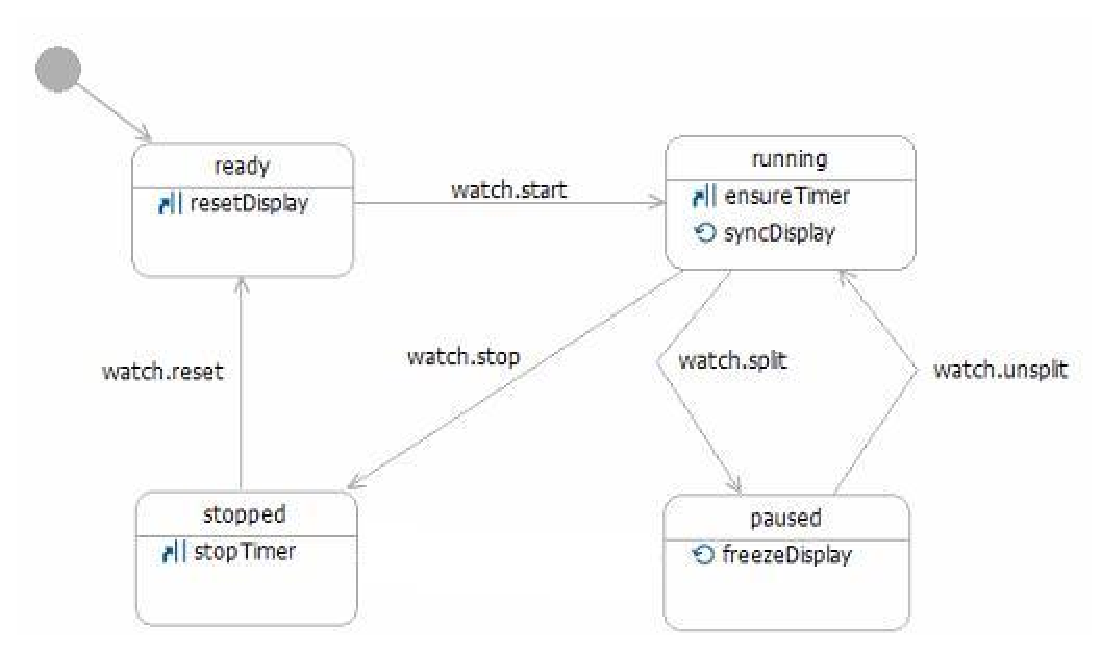
\includegraphics[height=8cm]{img/stopwatch}
   \caption{state chart diagram that describes the behavior of this particular stopwatch}
\end{figure}

\subsubsection{Model specification}

This current implementation has several differences from the original model from the Apache Commons website\cite{Apache}, however most states and transitions will remain as in the original model.

Several new custom actions will be implementated: 

\begin{itemize}
   \item \textsf{ResetDisplay:} As entry action of "reset" state. This action should set to zero the counter. 
   \item \textsf{FreezeDisplay:} As entry action of the "paused" state. The action should log a message.
   \item \textsf{StopTimer:} As entry action of the "stopped" state. The action should log a message. 
\end{itemize}

Also the startTimer activity will be added to the \textsf{running} state, which starts a thread responsible for counting the ticks. When the state Machine exits the \textsf{running} state, the thread is deleted terminated. 

The events (\textsf{start}, \textsf{stop}, \textsf{split}, \textsf{unsplit}, \textsf{reset}) will be CORBA calls which can be invoked by other ACS components or clients. The handling of the CORBA calls will inject the SCXML events (basically strings) into the SCXML engine. 

\subsubsection{SCXML document}

This file must specify the state machine behavior. SCXML documents (more generically, UML state chart diagrams) can be used to define stateful behavior of objects and Commons SCXML enables developers to take this model directly into the corresponding code artifacts (in this case using a Model Independent Engine). The resulting artifacts tend to be much simpler, embodying an useful separation of concerns and are easier to understand and maintain.

\lstset{
language=Java,
basicstyle=\footnotesize,
breaklines=true,
%numbers=left,
numberstyle=\footnotesize,
frame=single
}

\begin{lstlisting}
<scxml xmlns="http://www.w3.org/2005/07/scxml"
       version="1.0"
       xmlns:my1="http://my.custom-actions.domain/CUSTOM1"
       xmlns:my2="http://my.custom-actions.domain/CUSTOM2"
       xmlns:my3="http://my.custom-actions.domain/CUSTOM3"
       initialstate="reset">

    <state id="reset">
        <onentry>
            <my1:resetDisplay name="world" />
        </onentry>
        <transition event="watch.start"   target="running"/>
    </state>

    <state id="running">
        <invoke targettype="java" src="foo"/>
        <transition event="watch.split"   target="paused"/>
        <transition event="running.invoke.done" target="stopped"/>
    </state>

    <state id="paused">
        <onentry>
            <my2:freezeDisplay name="world" />
        </onentry>
        <transition event="watch.unsplit" target="running"/>

    </state>

    <state id="stopped">
        <onentry>
            <my3:stopTimer name="world" />
        </onentry>
        <transition event="watch.reset"   target="reset"/>
    </state>

</scxml>
\end{lstlisting}


According to the new model specifications, custom actions have been added in the \textsf{<onentry>} wrapper from some states, which contains executable content to be executed when the state is entered. Generally actions can be used where "executable content" is permissible, also within \textsf{<onexit>} and \textsf{<transition>} elements.

Each custom action must be defined in a fictitious namespace inside the \textsf{<scxml>} wrapper, like for example the \textsf{"http://my.custom-actions.domain/CUSTOM"}.

Also, the activities will be added using the \textsf{<invoke>} interface, that deals with the invocation of activities associated with a particular state in the state machine.

The XML file must be added in the \textsf{scxml-component/src/alma/STOPWATCH\_MODULE/ StopWatchImpl/config} folder. The file stopwatch.xml will be taken as an extra file, so it must be defined in the Makefile as follows. 


\begin{lstlisting}
	StopWatchImpl_EXTRAS=alma/STOPWATCH_MODULE/StopWatchImpl/config
\end{lstlisting}

\subsection{Integrating ACS and Apache Commons SCXML}

The component root directory will be \textsf{/scxml-component}. A simple way to create it using the pre-defined standard directory structure is by using the command: 

\begin{lstlisting}
	getTemplate 
\end{lstlisting}	

Which provides differents templates. In this case we are interested in choosing the option directoryStructure. Then we choose the option create \textsf{WS\_MODROOT} area thats create the directory structure type for the software source code. Each \textsf{MODROOT} corresponds to a software module containing a set of standard subdirectories. 

\subsubsection{Creating IDL}

A component’s functional interface must be specified in CORBA’s Interface Definition Language (IDL). According to the ALMA directory structure, the IDL files must be put in \textsf{/scxml-component/idl/} foder. In that place the StopWatch.idl file must be defined with the following structure. 


\begin{lstlisting}
#ifndef _STOPWATCH_IDL_
#define _STOPWATCH_IDL_

#include <acscomponent.idl>
#pragma prefix "alma"

module STOPWATCH_MODULE
{
        interface  StopWatch : ACS::ACSComponent
   {
      string getDisplay();
      string getCurrentState();
      boolean fireEvent(in string event);
      boolean start();
      boolean stop();
                boolean split();
      boolean unsplit();
                boolean reset();
   };
};

\end{lstlisting}	

In this file the module with the name \textsf{STOPWATCH\_MODULE} was defined. Inside it, the StopWatch interface methods are declared, which can be invoked for other components or clients.

After the IDL file has been written, a couple of Java classes must be generated from it, so it is necessary to add the following line to the ALMA Makefile option in the \textsf{/scxml-component/src/} folder. 

\begin{lstlisting}
	IDL_FILES = StopWatch
\end{lstlisting}	

\subsubsection{Custom Actions Implementation}

The custom actions must be implemented in an independent Java class, in the same project package (could be a different one as well), which must extend the Commons SCXML Action abstract base class. 

\begin{lstlisting}
package alma.STOPWATCH_MODULE.StopWatchImpl;

import java.util.logging.Logger;

import java.util.Collection;
import org.apache.commons.logging.Log;
import org.apache.commons.scxml.ErrorReporter;
import org.apache.commons.scxml.EventDispatcher;
import org.apache.commons.scxml.SCInstance;
import org.apache.commons.scxml.SCXMLExpressionException;
import org.apache.commons.scxml.model.Action;
import org.apache.commons.scxml.model.ModelException;

public class ResetDisplay extends Action
{
      /** Serial version UID. */
      private static final long serialVersionUID = 1L;
      /** This is who we say hello to. */
      private String name;
      /** We count callbacks to execute() as part of the test suite. */
     public static int callbacks = 0;
 
      /** Public constructor is needed for the I in SCXML IO. */
      public ResetDisplay() {
          super();
      }
  
      /**
       * Get the name.
       *
       * @return Returns the name.
       */
      public String getName() {
          return name;
      }
  
      /**
       * Set the name.
       *
       * @param name The name to set.
          */
      public void setName(String name) {
          this.name = name;
      }
  
      /**
       * @inheritDoc
       */
      public void execute(final EventDispatcher evtDispatcher, final ErrorReporter errRep, final SCInstance scInstance, final Log appLog, final Collection derivedEvents)
      throws ModelException, SCXMLExpressionException {
        
         ((StartTimer) scInstance.getRootContext().get("tictac")).reset();
         ((Logger) scInstance.getRootContext().get("logger")).info("CustomAction::resetDisplay()");
      }
}
\end{lstlisting}	

The execute() method contains the action to perform. This custom action must reset the Timer thread and log it.

All custom actions implementated have a similar structure, so we show only one for demonstration purposes. 

The activities that will be invoked and then executed by the engine must be defined like a common java class. In our example the activity will be a thread process that controls the stopwatch tics and then, when the engine sends the flow control out of the parent's running state, the thread must be joined.

It is important to remember that to implement a thread in a java the class needs to extend the Thread class or implement the Runnable interface. Furthermore,the class requires the run method to be implemented.

The source code of the class is the following 

\begin{lstlisting}
package alma.STOPWATCH_MODULE.StopWatchImpl;

import java.util.Timer;
import java.util.TimerTask;

import org.apache.commons.scxml.SCXMLExecutor;

public class StartTimer extends Thread
{
    SCXMLExecutor exec;
    /** The events for the stop watch. */
    public static final String EVENT_START = "watch.start",
        VENT_STOP = "watch.stop", EVENT_SPLIT = "watch.split",
        EVENT_UNSPLIT = "watch.unsplit", EVENT_RESET = "watch.reset";

    public static StringBuffer stringBuffer;

    /** The fragments of the elapsed time. */
    private static int hr, min, sec, fract;
    /** The fragments of the display time. */
    private static int dhr, dmin, dsec, dfract;
    /** The stopwatch "split" (display freeze). */
    private static boolean split;
    /** The Timer to keep time. */
    private static Timer timer;
    /** The display decorations. */
    private static final String DELIM = ":", DOT = ".", EMPTY = "", ZERO = "0";

    public void run(){ 
        split = false;
        if (timer == null) {
            timer = new Timer(true);
            timer.scheduleAtFixedRate(new TimerTask() {
                public void run() {
                    increment();
                }
            }, 100, 100);
        }
    }
 
    public synchronized void stopping() {
        timer.cancel();
        timer = null;

    }

    public synchronized void paussing() {
        split = true;
    }

    private void increment() {
        if (fract < 9) {
            fract++;
        } else {
            fract = 0;
            if (sec < 59) {
                sec++;
            } else {
                sec = 0;
                if (min < 59) {
                    min++;
                } else {
                    min = 0;
                    if (hr < 99) {
                        hr++;
                    } else {
                        hr = 0; //wrap
                    }
                }
            }
        }
        if (!split) {
            dhr = hr;
            dmin = min;
            dsec = sec;
            dfract = fract;
        }
    }

    public void running() {
        split = false;
        if (timer == null) {
            timer = new Timer(true);
            timer.scheduleAtFixedRate(new TimerTask() {  public void run() { increment();} }, 100, 100);
        }
    }

    public static String getDisplay() {
        String padhr = dhr > 9 ? EMPTY : ZERO;
        String padmin = dmin > 9 ? EMPTY : ZERO;
        String padsec = dsec > 9 ? EMPTY : ZERO;
        stringBuffer = new StringBuffer();
        return stringBuffer.append(padhr).append(dhr).append(DELIM).
            append(padmin).append(dmin).append(DELIM).append(padsec).
            append(dsec).append(DOT).append(dfract).toString();
    }

    public static void reset() {
        hr = min = sec = fract = dhr = dmin = dsec = dfract = 0;
        split = false;
    }

}

\end{lstlisting}

All the methods implemented in this class that takes care of the functionality of the stopwatch were based on the original use case from the Apache Commons SCXML website\cite{Apache}. 

\subsubsection{Invoker Implementation}

To define the interaction (bi-directional events pipe) between the parent sate machine and the activities that we will define we need to use the Invoker interface.

Invocable activities must first register an Invoker implementation class for the appropriate \textsf{type} (attribute of ) with the parent SCXMLExecutor. This implementation must ensure that, when activities are completed, it must fire a \textsf{done} event.

The name of the special \textsf{done} event must be the ID of the parent state wherein the corresponding resides, with the String \textsf{.invoke.done} appended. 

The implemented \textsf{JavaInvoker} class looks like this. 

\begin{lstlisting}

package alma.STOPWATCH_MODULE.StopWatchImpl;

import java.util.Map;
import alma.acs.container.ContainerServices;

import org.apache.commons.scxml.SCInstance;
import org.apache.commons.scxml.TriggerEvent;
import org.apache.commons.scxml.model.ModelException;
import org.apache.commons.scxml.invoke.Invoker;
import org.apache.commons.scxml.invoke.InvokerException;

public class JavaInvoker implements Invoker
{
     private String parentStateId;
     private SCInstance parentSCInstance;
     public  Thread th;
     public static StartTimer tictac;
     public ContainerServices _containerServices;

     public JavaInvoker()
     {
     }     

     public void setParentStateId(final String parentStateId) {
         this.parentStateId = parentStateId;
     }

     public void setSCInstance(final SCInstance scInstance) {
         this.parentSCInstance = scInstance;
         _containerServices = (ContainerServices) this.parentSCInstance.getRootContext().get("containerServices");
     }

     public void invoke(final String source, final Map params) throws InvokerException {
      try {
         tictac = new StartTimer();
         this.parentSCInstance.getRootContext().set("tictac", tictac);
         th = _containerServices.getThreadFactory().newThread(tictac);
         th.start();
        } catch (Exception e) {
            e.printStackTrace();
        }
     }

     public void parentEvents(TriggerEvent[] events) throws InvokerException {
        if (events[0].getName().equals("watch.stop") && (parentStateId.equals("running")))  {
           try {
             tictac.stopping();
             th.join();
             parentSCInstance.getExecutor().triggerEvent(new TriggerEvent(parentStateId + ".invoke.done", TriggerEvent.SIGNAL_EVENT));
           } catch (ModelException me) {
              throw new InvokerException(me.getMessage(), me.getCause()); }
             catch (Exception e){
      }
        }
        if (events[0].getName().equals("watch.split") && parentStateId.equals("running")) {
           try {
               tictac.paussing();
           } catch (Exception e) { 
        }
     }
    }

     public void cancel() throws InvokerException {
      System.out.println("In Cancel for ID " + parentStateId);
     }
 }

\end{lstlisting}	

Note that inside the \textsf{invoke} method the Java thread instance is created using the instance of Thread ACS class.

The method parentEvent forwards the events triggered on the parent state machine to the invoked activity. 

\subsubsection{Component Implementation}

By convention, we call the implementation class StopWatchImpl and it must define the functional interface methods and the component lifecycle interface that the container uses to start and stop the ACS component and provide a callback handle. 

First we need to re-define the module package according to the subpackage-per-component-implementation convention that ACS uses. 

\begin{lstlisting}
	package alma.STOPWATCH_MODULE.StopWatchImpl; 
\end{lstlisting}	

Then, we must import the ACS packages (ComponentState , LifeCycle , LifeCycleException , ContainerServices ) and the functional methods interfaces of the module, as well as the java packages that will be used. 

\begin{lstlisting}

import alma.acs.component.ComponentLifecycle;
import alma.acs.component.ComponentLifecycleException;
import alma.acs.container.ContainerServices;
import alma.ACS.ComponentStates;
import alma.STOPWATCH_MODULE.StopWatchOperations;

import java.util.Set;
import java.util.List;
import java.util.ArrayList;
import java.util.logging.Logger;
import java.io.IOException;
import java.net.URL;

\end{lstlisting}

Also Apache commons SCXML packages must be imported, which provides a generic state-machine based execution environment (Developer should have installed it previously ).

\begin{lstlisting}
import org.xml.sax.ErrorHandler;
import org.xml.sax.SAXException;
import org.apache.commons.scxml.model.CustomAction;
import org.apache.commons.scxml.model.ModelException;
import org.apache.commons.scxml.model.SCXML;
import org.apache.commons.scxml.SCXMLExecutor;
import org.apache.commons.scxml.TriggerEvent;
import org.apache.commons.scxml.io.SCXMLParser;
import org.apache.commons.scxml.Context;
import org.apache.commons.scxml.Evaluator;
import org.apache.commons.scxml.env.jexl.JexlContext;
import org.apache.commons.scxml.env.jexl.JexlEvaluator;
import org.apache.commons.scxml.env.SimpleDispatcher;
import org.apache.commons.scxml.env.SimpleErrorReporter;
import org.apache.commons.scxml.env.SimpleSCXMLListener;
import org.apache.commons.logging.Log;
import org.apache.commons.logging.LogFactory;

\end{lstlisting}	

It should be noted that, unlike the basic pre-deploymentated stopwatch, in this example we do not use the abstract class \textsf{AbstractStateMachine} mainly due to it limiting the operation of the advanced elements of the API. 

The definition of the class \textsf{StopWatchImpl} must implement the operations defined in the IDL file and the lifecycle interface. 

\begin{lstlisting}
public class StopWatchImpl implements StopWatchOperations , ComponentLifecycle , Runnable
\end{lstlisting}

Variables and class definition.

We need to define Apache Commons SCXML and ACS variables that we use in our code. 
	
\begin{lstlisting}
    /////////////////////////////////////////////////////////////
    // State Machine Apache Commons SCXML variables
    /////////////////////////////////////////////////////////////

    private ErrorHandler errorHandler;
    // The state machine that will drive the instances of this class.
    private SCXML scxml = null;
    // The instance specific SCXML engine.
    private SCXMLExecutor engine;

    private SimpleSCXMLListener listener = new SimpleSCXMLListener();
    // The log
    private Log log;
  
    private URL urlsc;

    /////////////////////////////////////////////////////////////
    // ACS component variables
    /////////////////////////////////////////////////////////////

    private ContainerServices _containerServices;
    private Logger _logger;

\end{lstlisting}

The Apache Commons SCXML variables are:
\begin{itemize}
    \item \textsf{errorHandler} is a instance of the ErrorHandler interface for SAX error handlers.
    \item \textsf{scxml} represents the object model that corresponds to the !< scxml !> root element, and serves as the "document root".
    \item \textsf{engine} that is the engine that runs the state machine.
    \item \textsf{listener} that logs execution.
    \item \textsf{log} that logs execution.
    \item \textsf{urlsc} that is a instance of the URL, that represents a canonical absolute URL to parse (relative URLs within the top level document are to be resovled against this URL). 
\end{itemize}

The ACS variables are: 
\begin{itemize}
    \item \textsf{\_containerServices} that is the reference to the ContainerServices object that the container will give us.
    \item \textsf{\_logger} reference to the logger object which we'll get from the container. 
\end{itemize}

Inside the class constructor we invoke the \textsf{setUpStateMachine()} method that is in charge of defining the custom actions to use and parsing the SCXML document into the Java object model (\textsf{scxml} variable) provided in the model package, using the SCXMLParser, which is part of the core Commons SCXML API. 

\begin{lstlisting}
private void setUpStateMachine() {
        /** Creation of custom Actions */
        CustomAction ca1 = new CustomAction("http://my.custom-actions.domain/CUSTOM1", "resetDisplay", ResetDisplay.class);
        CustomAction ca2 = new CustomAction("http://my.custom-actions.domain/CUSTOM2", "freezeDisplay", FreezeDisplay.class);
        CustomAction ca3 = new CustomAction("http://my.custom-actions.domain/CUSTOM3", "stopTimer", StopTimer.class);
        List <CustomAction> customActions = new ArrayList <CustomAction> ();
        customActions.add(ca1);
        customActions.add(ca2);
        customActions.add(ca3);

        urlsc = this.getClass().getClassLoader().getResource("alma/STOPWATCH_MODULE/StopWatchImpl/config/stopwatch.xml");
        try {
            scxml = SCXMLParser.parse(urlsc, errorHandler, customActions);
            }
        catch (IOException ioe) {
            logError(ioe);
        } catch (SAXException sae) {
            logError(sae);
        } catch (ModelException me) {
            logError(me);
        } catch (Exception e) {
        }
    }
\end{lstlisting}

As already mentioned, besides the functional methods, we must add the \textsf{ComponentLifeCycle} implementation and Component methods as following. 

\begin{lstlisting}
  /////////////////////////////////////////////////////////////
    // Implementation of ComponentLifecycle
    /////////////////////////////////////////////////////////////
    
    public void initialize(ContainerServices containerServices) throws ComponentLifecycleException {
         _containerServices = containerServices;
         _logger = _containerServices.getLogger();
         _logger.info("initialize() called...");
    }
    
    public void execute() {
         _logger.info("execute() called...");
         initializeStateMachine(scxml, new JexlContext(), new JexlEvaluator());
    }
    
    public void cleanUp() {
         _logger.info("cleanUp() called");
    }
    
    public void aboutToAbort() {
         cleanUp();
         _logger.info("managed to abort...");
    }

    /////////////////////////////////////////////////////////////
    // Implementation of ACSComponent
    /////////////////////////////////////////////////////////////
    
    public ComponentStates componentState() {
       return _containerServices.getComponentStateManager().getCurrentState();
    }
    public String name() {
       return _containerServices.getName();
    }

    public void run() {
   _logger.info("run...");
    }

\end{lstlisting}

After the  \textsf{initialize()} method has returned, the method  \textsf{execute()} will be called by the container. Inside it, the  \textsf{initializeStateMachine()} method it will be invoked. 

\begin{lstlisting}
    private void initializeStateMachine(final SCXML stateMachine, final Context rootCtx, final Evaluator evaluator) {
       engine = new SCXMLExecutor(evaluator, new SimpleDispatcher(), new SimpleErrorReporter());
       engine.setStateMachine(stateMachine);
       rootCtx.set("containerServices", (ContainerServices) _containerServices);
       rootCtx.set("logger", (Logger) _logger);
       engine.setRootContext(rootCtx);
       engine.addListener(stateMachine, listener);
       engine.registerInvokerClass("java", JavaInvoker.class);
       try {
            engine.go();
        } catch (ModelException me) {
        } catch (Exception e){
               e.printStackTrace();
        }
    }
\end{lstlisting}

Inside this method, we first create an instance of the Commons SCXML executor, which is the engine that runs the state machine. The Context and Evaluator parameters, are interfaces that serve as adapters to the particular expression language API. Then we must add to it the Java object model already created in the \textsf{setUpStateMachine()} method.

The "scope" of the state machine implementation is defined by the \textsf{Context} variable. Each element within an SCXML document gets its own \textsf{Context} or variable scope.

The ACS variables \textsf{\_containerServices} and \textsf{\_logger} are added to the context, so they can be be used in all classes that make up the implementation of state machine model. Then the context is added to the engine.

It is also necessary to add to the engine the Listener interface, that will control observable entities in the SCXML model. Observable entities include SCXML instances (subscribe to all entry, exit and transition notifications), State instances (subscribe to particular entry and exit notifications) and Transition instances (subscribe to particular transitions). For our example is not necessary to use a very particular implementation and, for this reason, an instance of the class \textsf{SimpleSCXMLListener} is used, which logs the executions.

The implementated Java Invoker must be added to the engine through the \textsf{engine.registerInvokerClass()} method, where the arguments specify the target type (specified by "type" attribute of tag in the SCXML document) and the invoker class.

Finally we must specify in the makefile the name and the path where the files of our implementation can be found. 

\begin{lstlisting}
JARFILES= StopWatchImpl
StopWatchImpl_DIRS=alma/STOPWATCH_MODULE/StopWatchImpl
\end{lstlisting}

\subsubsection{Component Helper Clases}

The Stopwatch component needs its corresponding helper class. A template for the helper class gets generated by the build system if the Makefile in the /scxml-component/src/ folder contain the following lines:

\begin{lstlisting}
COMPONENT_HELPERS=on
\end{lstlisting}

The template will be generated in the \textsf{scxml-component/src/alma/STOPWATCH\_MODULE/ StopWatchImpl/} folder. For our example the class does not need to be modified and we only need to remove the .tpl ending. 

\subsubsection{Configuration DataBase}

The CDB file must be defined in the \textsf{scxml-component/test/CDB directory} . Our example will be a component defined statically, so we need to add new lines in the \textsf{MACI/Components/Components.xml} file with the component name STOPWATCH, the component helper class, the CORBA interface respository ID of the component's IDL and the name of the container that will be used by the ACS Manager to deploy it. The entire file looks like this: 

\begin{lstlisting}
<?xml version="1.0" encoding="ISO-8859-1"?>
<Components  xmlns="urn:schemas-cosylab-com:Components:1.0"
       xmlns:cdb="urn:schemas-cosylab-com:CDB:1.0" 
       xmlns:baci="urn:schemas-cosylab-com:BACI:1.0" 
       xmlns:xsi="http://www.w3.org/2001/XMLSchema-instance">

      <_ Name="STOPWATCH"
         Code="alma.STOPWATCH_MODULE.StopWatchImpl.StopWatchHelper"
         Type="IDL:alma/STOPWATCH_MODULE/StopWatch:1.0"
         Default="true"
         Container="frodoContainer" ImplLang="java" />
</Components>
\end{lstlisting}

In this step it is neccesary to reset the \textsf{ACS\_CDB} environment variable with the absolute path where it is defined. For example. 
\begin{lstlisting}
export ACS_CDB =/diska/home/almadev/GSME/stopwatchComponent/test 
\end{lstlisting}

\subsubsection{Client}

We can use the ACS Tool \textsf{ObjectExplorer} as a generic client for all components. It runs with the command: 

\begin{lstlisting}
objexp
\end{lstlisting}
\addcontentsline{toc}{section}{References}

\clearpage
\bibliographystyle{plain}
\bibliography{ref}		
\end{document}
